    \documentclass[xcolor=dvipsnames]{beamer}
\usecolortheme[named=Brown]{structure}
\usetheme{Malmoe}
\useoutertheme{infolines}
% All the information about beamer themes comes from here
% http://en.wikibooks.org/wiki/LaTeX/Presentations

\usepackage{ross}

\usepackage{tikz}
\usetikzlibrary{calc}
\usepackage{pgfplots}
\pgfplotsset{width=7cm,compat=1.8}

%Information for the title slide
\title{Deformations of Harmonic Maps}
\author{Ross Ogilvie}
\institute[]{
  School of Mathematics and Statistics\\
  University of Sydney
  }
\date{July 2015}

% This puts a table of contents showing where you are up to at the start of every section
% \AtBeginSection[]
% {
%   \begin{frame}
%     \frametitle{Table of Contents}
%     \tableofcontents[currentsection]
%   \end{frame}
% }

%gets rid of navigation symbols, which are stupid
\setbeamertemplate{navigation symbols}{}

%%%%%%%%%%%%%%%%%
% Document starts
%%%%%%%%%%%%%%%%%
\begin{document}
\begin{frame}
    \titlepage
\end{frame}


\begin{frame}{The spaces}
\begin{itemize}
\item A torus is a doughnut.
\begin{center}

\includegraphics[width=50mm,scale=0.1]{simpsons-donut.png}
\end{center}
\item A 3-sphere $\S^4$ is unit sphere in $\R^4$ or $\C^2$. For us, we will think of it as $SU(2)$, which looks like
\[
\begin{pmatrix} α & -\bar{β} \\ β & \bar{α} \end{pmatrix},\text{ with } α\bar{α} + β\bar{β} = 1
\]
\end{itemize}
\end{frame}


\begin{frame}{Harmonic Map}
\begin{itemize}
\item Let $f : T^2 \to SU(2)$. Use $f$ to pull pack the connection on $SU(2)$ to get a connection $A$. Automatically we have $d_A (df) = 0$.
\item A harmonic map is one that minimises the energy. It must satisfy $d_A^* (df) = 0$.
\item Translate the values of $df$ so it is a map to the Lie algebra, and split it up as $\tfrac{1}{2} f^{-1} df = Φ - Φ^*$.
\item We can then rearrange our two equations to be about $A$ and $Φ$.
\[
d^{''}_A Φ = 0,\qquad\qquad F_A = [Φ,Φ^*]
\]
$Φ$ is called the Higgs field.
\end{itemize}
\end{frame}

\begin{frame}{Family of Flat Connections}
\begin{itemize}
\item Given a pair $(Φ,A)$, we can make a family of connections in the following way. Let $ζ\in\C^\times$ and define
\[
\nabla_ζ := \nabla_A + ζ^{-1}Φ - ζ Φ^*
\]
\item Every connection in this family is flat (zero curvature) since
\[
F = (d_A + ζ^{-1}Φ - ζΦ^*)^2 = d_A^2 - [Φ,Φ^*] = 0
\]
\item The connections are $SL(2,\C)$ valued. When $ζ=1,-1$ the result is the left and right connections on $SU(2)$
\end{itemize}
\end{frame}


\begin{frame}{Holonomy}
\begin{itemize}
\item Because the connections are flat, we can define holonomy for them. Pick a base point, and take two loops around the torus.
\item Parallel translating a vector with $\nabla_ζ$ around one loop gives a linear map the vector space at the base point. Call this $H(ζ)$. Around the other loop call the transformation $\tilde H(ζ)$.
\item With some analysis and the fact that these two matrices commute (because the fundamental group of the torus is abelian), one can show that $(\tr H)^2 - 4$ (a function in $ζ$) vanishes to odd order only finitely many times.
\end{itemize}
\end{frame}
%
% \begin{frame}
% \begin{center}
% \begin{tikzpicture}
% \begin{axis}[axis lines=none]
% \addplot3[
%  surf,
%  colormap/blackwhite,
%  samples=20,
%  domain=0:2*pi,
%  y domain=0:2*pi,
%  z buffer=sort
% ]
% ( {(2+cos(deg(x)))*cos(deg(y))},
%  {(2+cos(deg(x)))*sin(deg(y))},
%  {sin(deg(x))}
% );
%  \addplot3 [domain=0:2*pi, samples y=0, red!70, smooth] ( {(2+cos(deg(x)))*cos(deg(y))},
%   {(2+cos(deg(x)))*sin(deg(y))},
%   {sin(deg(x))}
%  );
%  \addplot3 [domain=0:2*pi, samples y=0, blue!70, smooth] ( {(2+cos(deg(y)))*cos(deg(x))},
%   {(2+cos(deg(y)))*sin(deg(x))},
%   {sin(deg(y))}
%  );
% \addplot3[surf, colormap/cool, samples=10, domain=-2:2, y domain=0:1] ( {3}, {x}, {y} );
% \end{axis}
% \end{tikzpicture}
% \end{center}
% \end{frame}


\begin{frame}{Spectral Curve}
\begin{itemize}
\item The eigenvalues of $H(ζ)$ are $μ(ζ), μ(ζ)^{-1}$. The characteristic polynomial is
\[
μ^2 - (\tr H) μ + 1 = 0
\]
\item What we want to do is to build a curve over $ζ\in\C^\times$ where $μ$ is single valued.
\item We can use the characteristic equation to define a two sheeted cover of $\C^\times$ with finite branching.
\item Looking at the behaviour of $μ$ as $ζ\to 0$ (ditto $ζ\to\infty$), we can fill in the missing points to make a two sheeted cover $Σ$ of $\CP^1$, called the spectral curve.
\item It is an algebraic curve, with several nice additional structures.
\end{itemize}
\end{frame}


\begin{frame}{The Differentials}
\begin{itemize}
\item The spectral curve provides a natural setting to talk about the eigenvalues, but they are not so nice themselves.
\item However, $\log μ, \log \tilde {μ}$ are holomorphic on $\C^\times$, have simple poles above $ζ=0,\infty$ and nowhere else, but are only locally defined.
\item $d \log μ$ removes the additive ambiguity of $\log$. Thus we consider a pair of meromorphic differentials $Θ = d \log μ, \tilde {Θ} = \log \tilde {μ}$, which have residue free double poles over $ζ=0,\infty$.
\item In order for the eigenvalues to be well defined, one requires that the periods of the differentials lie in $2π\iu\Z$.
\end{itemize}
\end{frame}


\begin{frame}{Spectral Data}
\begin{itemize}
\item We now have a curve $Σ$ and a pair of differentials $Θ,\tilde{Θ}$. There is one more piece of information needed: a line bundle.
\item Then a theorem of Hitchin gives conditions for such data to correspond to a harmonic map.
\item An important part of this result is that for fixed $(Σ,Θ,\tilde{Θ})$ we can choose from many line bundles. These are called isospectral deformations.
\end{itemize}
\end{frame}


\begin{frame}{Genus Zero example}
\begin{itemize}
\item Take the spectral curve to be genus zero. By the various symmetric constraints, its two branch points must be a pair $α,\cji{α}$, with $α\in D$
\[
η^2 = P(ζ) = (ζ-α)(1-\bar{α}ζ)
\]
\item All differentials on it are exact, and for the $Θ$'s to have the right poles they must be of the form
\[
\log μ = (bζ^{-1} - \bar{b})η, \qquad b\in\C
\]
\item The constraints to be a harmonic map further imply that
\[
b = \frac{π}{2}\left( \frac{n}{\abs{1+α}} + \iu \frac{m}{\abs{1-α}} \right), \qquad n,m\in\Z
\]
\end{itemize}
\end{frame}


\begin{frame}{Genus Zero Example}
\begin{center}
  \begin{tikzpicture}
    \draw [thin, gray,-latex] (-3,0) -- (3,0);% Draw x axis
    \draw [thin, gray,-latex] (0,-3) -- (0,3);% Draw y axis

    \foreach \x in {-2,-1,...,2}{% Two indices running over each
      \foreach \y in {-3,-2,...,3}{% node on the grid we have drawn
        \node[draw,circle,inner sep=2pt,fill] at (1.5*\x,\y) {};
            % Places a dot at those points
      }
    }
    \draw [ultra thick,-latex,red] (Origin) -- (1.5,1);
    \draw [ultra thick,-latex,blue] (1.5,1) -- (0,2);
    \draw [ultra thick,-latex,blue] (Origin) -- (-1.5,1);
    \draw [ultra thick,-latex,red] (-1.5,1) -- (0,2);
  \end{tikzpicture}
\end{center}
\end{frame}


\begin{frame}{Moduli Space}
\begin{itemize}
\item In general, $Σ$ of genus $g$ curve can be described by $g+1$ pair of conjugate inverse points.
\item The differentials become much harder to pin down. However they must be of the form
\[
Θ = \frac{dζ}{ζ^2η} b(ζ)
\]
for some polynomials of degree $g+3$. If you just require symmetries and imaginary periods, there is a plane of differentials.
\item Whitham deformations tell us that the space of $(Σ,Θ,\tilde{Θ})$ is 2-dimensional.
\end{itemize}
\end{frame}

\begin{frame}{Genus One}
\begin{itemize}
\item Spectral curves have two pairs of branch points $α,β,\cji{α},\cji{β}$, $(α,β)\in D\times D \setminus Δ$.
\end{itemize}
\begin{center}
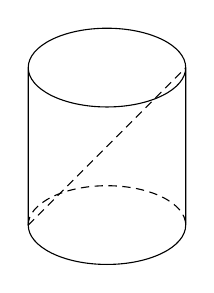
\begin{tikzpicture}
\draw (-1,2) -- (-1,0) arc (180:360:1cm and 0.5cm) -- (1,2) ++ (-1,0) circle (1cm and 0.5cm);
\draw[densely dashed] (-1,0) arc (180:0:1cm and 0.5cm);
\draw[densely dashed] (-1,0) -- (1,2);
\end{tikzpicture}
\end{center}
\end{frame}

\begin{frame}
\begin{itemize}
\item Period conditions mean that there are a collection of lines of differentials, one for each $2π\iu\Z$.
\end{itemize}

\begin{center}
  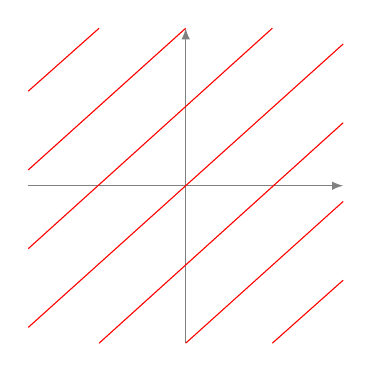
\begin{tikzpicture}
    \draw [thin, gray,-latex] (-2,0) -- (2,0);% Draw x axis
    \draw [thin, gray,-latex] (0,-2) -- (0,2);% Draw y axis

    \draw [red] (-2,-1.8) -- (2,1.8);
    \draw [red] (-2,-0.8) -- (1.1,2);
    \draw [red] (-2,0.2) -- (0,2);
    \draw [red] (-2,1.2) -- (-1.1,2);

    \draw [red] (-1.1,-2) -- (2,0.8);
    \draw [red] (0,-2) -- (2,-0.2);
    \draw [red] (1.1,-2) -- (2,-1.2);
  \end{tikzpicture}
\end{center}
\end{frame}

\begin{frame}
\begin{itemize}
\item Period conditions mean that there are a collection of lines of differentials, one for each $2π\iu\Z$.
\end{itemize}

\begin{center}
  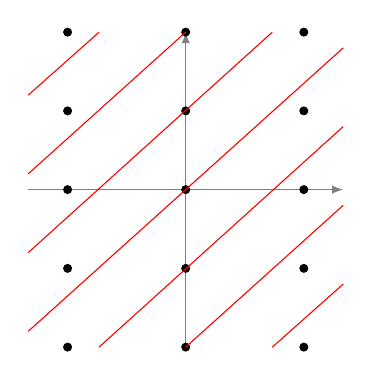
\begin{tikzpicture}
    \draw [thin, gray,-latex] (-2,0) -- (2,0);% Draw x axis
    \draw [thin, gray,-latex] (0,-2) -- (0,2);% Draw y axis

    \foreach \x in {-1,0,1}{% Two indices running over each
      \foreach \y in {-2,-1,0,1,2}{% node on the grid we have drawn
        \node[draw,circle,inner sep=1pt,fill] at (1.5*\x,\y) {};
            % Places a dot at those points
      }
    }
    \draw [red] (-2,-1.8) -- (2,1.8);
    \draw [red] (-2,-0.8) -- (1.1,2);
    \draw [red] (-2,0.2) -- (0,2);
    \draw [red] (-2,1.2) -- (-1.1,2);

    \draw [red] (-1.1,-2) -- (2,0.8);
    \draw [red] (0,-2) -- (2,-0.2);
    \draw [red] (1.1,-2) -- (2,-1.2);
  \end{tikzpicture}
\end{center}
\begin{itemize}
\item Not every spectral curve has differentials that meet all the conditions.
\item As one traverses around the diagonal, the lattice shifts.
\end{itemize}
\end{frame}


\begin{frame}
\begin{itemize}
\item On the exterior boundary, where one branch point lies in $\S^1$, normalisation of the spectral curve correspond to genus zero spectral data.
\end{itemize}
\begin{center}
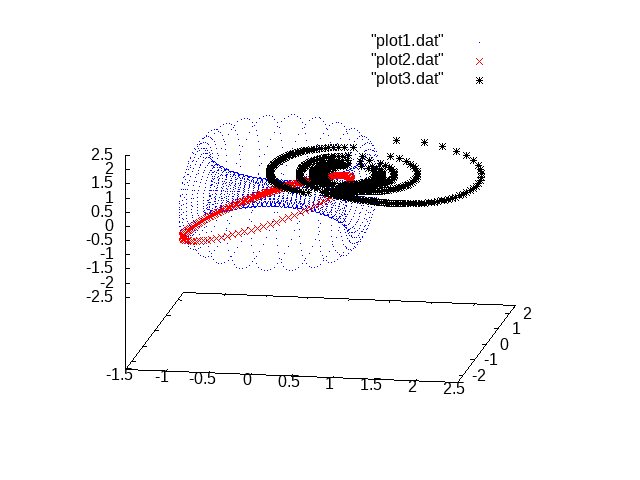
\includegraphics[width=100mm]{boundaryLink.png}
\end{center}
\end{frame}


\end{document}
